\chapter{The quantum harmonic oscillator}
\startcontents[chapters]
\printcontents[chapters]{}{1}{}
{\vspace{2em}\color{black}\titlerule[2pt]}
\vspace*{\fill}

%% introduction talk
\newpage
\columnratio{.7}

\section{Introduction}
%%
\subsection{Importance of the harmonic oscillator in physics}
The simplest example is a particle of mass $m$ moving in a potential which depends only on $x$ and has the form 
\begin{align*}
    V(x)=\frac{1}{2}kx^2,\quad k>0.
\end{align*}
\begin{figure}[h!]
    \centering
    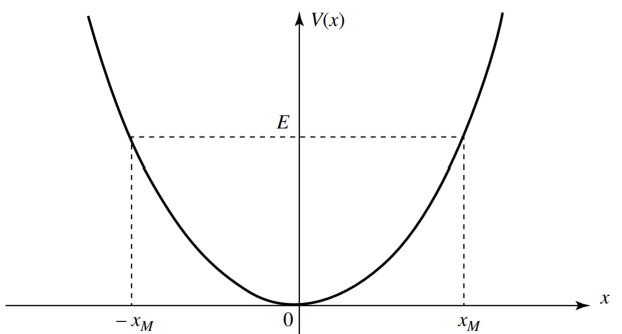
\includegraphics[width=.5\columnwidth]{PartOne/ChapterThree/potentialharmonicoscillator.png}
    \caption{Potential energy $V(x)$ of a 1D harmonic oscillator.}
\end{figure}
The particle is attracted towards the $x=0$ by a restoring force:
\begin{align*}
    F_x=\frac{dV}{dx}=-kx.
\end{align*}
In classical mechanics, the motion of the particle is a sinusoidal oscillation about $x=0$ with angular frequency $\omega=\sqrt{k/m}$.

\begin{emphasizer}[Various systems are governed by the harmonic oscillator equations]
    Whenever one studies the behavior of a system in the neighborhood of a stable equilibrium position, one arrives at equations which, 
    in the limit of small oscillations, are those of a harmonic oscillator.
\end{emphasizer}
%%
\subsection{The harmonic oscillator in classical mechanics}
The motion of the particle is governed by the dynamics equation
\begin{align}
    m\frac{d^2x}{dt^2}=-\frac{dV}{dx}=-kx\longrightarrow x=x_M\cos(\omega t-\varphi).
\end{align}
The kinetic energy of the particle is 
\begin{align}
    T=\frac{1}{2}m\left(\frac{dx}{dt}\right)^2=\frac{p^2}{2m},
\end{align}
where $p=mv$ is the momentum of the paticle. The total energy after substitution of $x_M$ is
\begin{align*}
    E=T+V=\frac{p^2}{2m}+\frac{1}{2}m\omega^2x^2=\frac{1}{2}m\omega^2x^2_M.
\end{align*}

\begin{itemize}[itemsep=0pt,topsep=0pt]
    \item The potential can be expanded in Taylor's series around $x_0$:
    \begin{align*}
        V(x)=\underbrace{V(x_0)}_{a}+V'(x_0)(x-x_0)+\underbrace{\frac{1}{2!}V^{(2)}(x_0)}_{b}(x-x_0)^2+\underbrace{\frac{1}{3!}V^{(3)}(x_0)}_{c}(x-x_0)^3+\cdots
    \end{align*}
    The force derived from the potential in the neighborhood of $x_0$ is 
    \begin{align}
        F_x=-\frac{dV}{dx}=-2b(x-x_0)-3c(x-x_0)^2+\cdots
    \end{align}
    The point $x=x_0$ is a stable equilibrium for the particle: $F_x(x_0)=0$. In adittion, if the amplitude of the motion of the particle 
    about $x_0$ is sufficiently small, we can keep with the linear term only and we have a harmonic oscillator since the dynamics equation can be approximated by 
    \begin{align*}
        m\frac{d^2x}{dt^2}\approx-2b(x-x_0).
    \end{align*}
    For higher energies $E$, the particle will be in period but not sinusoidal motion (as signal in Fourier series) between the limits $x_1$ and $x_2$. We then say that we are dealing with an \bfemph{anharmonic oscillator}.
    \begin{figure}[h!]
        \centering
        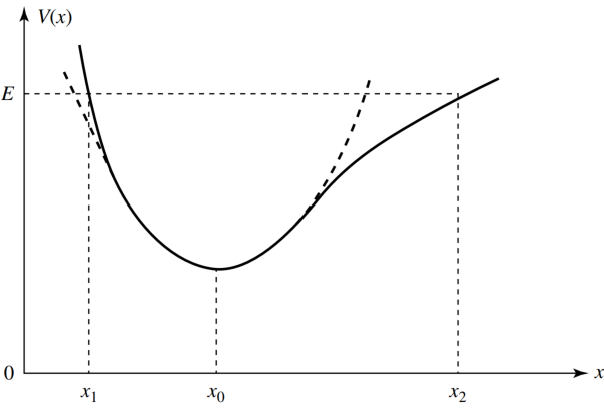
\includegraphics[width=.5\columnwidth]{PartOne/ChapterThree/taylorpotential.png}
        \caption{Any potential can be approximated by a parabolic potential. In $V(x)$, a classical particle of energy $E$ oscillates between $x_1$ and $x_2$.}
    \end{figure}
\end{itemize}
%
\subsection{General properties of the quantum mechanical Hamiltonian}
In QM, the classical quantities $x$ and $p$ are replaced respectively by the observables $X$ and $P$, which satisfy 
\begin{align*}
    [X,P]=i\hbar.
\end{align*}
It is then easy to obtain the Hamiltonian operator of the system from the total energy
\begin{align*}
    H=\frac{P^2}{2m}+\frac{1}{2}m\omega^2X^2.
\end{align*}
Since $H$ is time-independent (conservative system), the quantum mechanical study of the harmonic oscillator reduces to the solution of the eigenequation:
\begin{align*}
    H\ket{\varphi}=E\ket{\varphi}
\end{align*}
which is written, in the $\{\ket{x}\}$ representation 
\begin{align*}
    \left[-\frac{\hbar^2}{2m}\frac{d^2}{dx^2}+\frac{1}{2}m\omega^2x^2\right]\varphi(x)=E\varphi(x).
\end{align*}
Let us indicate some properties of the potential function:
\begin{itemize}[itemsep=0pt,topsep=0pt]
    \item\textbf{The eigenvalues of the Hamiltonian are positive}. If $V(x)$ has a lower bound, the eigenvalues $E$ of $H$ are greater than the minimum of $V(x)$:
    \begin{align*}
        V(x)\leq V_m\quad\text{requires}\quad E>V_m.
    \end{align*}
    We have chosen for the harmonic oscillator that $V_m=0$.
    \item\textbf{The eigenfunctions of $H$ have a definite parity} due to that $V(-x)=V(x)$ is an even function. We shall see that the eigenvalues of $H$ are not degenerate;
    the wave functions associated with the stationary tates are necessarily either even or odd.
    \item\textbf{The energy spectrum is discrete}. 
\end{itemize}
\section{Eigenvalues of the Hamiltonian}
%
\subsection{Notation}
It is easy to see that the observables $\hat{X}$ and $\hat{P}$ 
\begin{align*}
    \text{Dimensionless observables}\qquad\highlight{\hat{X}=\frac{X}{\sigma},\quad\hat{P}=\frac{\sigma P}{\hbar},\quad\text{where}\quad\sigma=\sqrt{\frac{\hbar}{m\omega}}=\text{Oscillator length $(m)$}}.
\end{align*}
are dimensionless. With these new operators, the canonical commutation is 
\begin{align}
    \text{Canonical commutation}\qquad\highlight{[\hat{X},\hat{P}]=i}
\end{align}
and the Hamiltonian can be put in the form 
\begin{align}
    H=\hbar\omega\hat{H},\quad\text{with}\quad \hat{H}=\frac{1}{2}(\hat{X}^2+\hat{P}^2).
\end{align}
In consequence, we seek the solutions of the following eigenequation
\begin{align*}
    \hat{H}\ket{\varphi_\nu^i}=\epsilon_\nu\ket{\varphi_\nu^i},
\end{align*}
where the operator $\hat{H}$ and the eigenvalues $\epsilon_\nu$ are \textbf{dimensionless}.

If $\hat{X}$ and $\hat{P}$ were numbers and not operators, we could write the sum $\hat{X}^2+\hat{P}^2$ appearing in the definition of $\hat{H}$ in the form of a product 
$(\hat{X}-i\hat{P})(\hat{X}+i\hat{P})$. However, the introuction of operators proportional to $\hat{H}\pm i\hat{P}$ enables us to simplify considerably out search for eigenvalues 
and eigenvectors of $\hat{H}$.
We therefore set 
\begin{align}
    \begin{array}{l}
        a=\dfrac{1}{\sqrt{2}}(\hat{X}+i\hat{P})\\
        a^\dagger=\dfrac{1}{\sqrt{2}}(\hat{X}-i\hat{P})
    \end{array}\Longleftrightarrow
    \begin{array}{l}
        \hat{X}=\dfrac{1}{\sqrt{2}}(a^\dagger+a)\\
        \hat{P}=\dfrac{i}{\sqrt{2}}(a^\dagger-a)
    \end{array}.
\end{align}
The commutator of $a$ and $a^\dagger$ is 
\begin{align}
    [a,a^\dagger]=\frac{1}{2}[\hat{X}+i\hat{P},\hat{X}-i\hat{P}]=\frac{i}{2}[\hat{P},\hat{X}]-\frac{i}{2}[\hat{X},\hat{P}]=1\longrightarrow\highlight{[a,a^\dagger]=1}.
\end{align}
If we do $aa^\dagger$ we obtain
\begin{align*}
    a^\dagger a=\frac{1}{2}(\hat{X}-i\hat{P})(\hat{X}+i\hat{P})=\frac{1}{2}(\hat{X}^2+\hat{P}^2+i\hat{X}\hat{P}-i\hat{P}\hat{X})=\frac{1}{2}(\hat{X}^2+\hat{P}^2-1).
\end{align*}
Comparing with $\hat{H}$ we see that 
\begin{align*}
    \highlight{\hat{H}=a^\dagger a+\frac{1}{2}=aa^\dagger-\frac{1}{2}}.
\end{align*}
We see that we canot put $\hat{H}$ in a product of linear terms, due to the non-commutatitivty of $\hat{X}$ and $\hat{P}$ ($1/2$ term).

We introduce another operator:
\begin{align}
    \text{Operator $N$}\qquad\highlight{N=a^\dagger a}.
\end{align}
This operator is Hermitian 
\begin{align}
    N^\dagger=a^\dagger(a^\dagger)^\dagger=a^\dagger a=N.
\end{align}
And its relation with $\hat{H}$ is 
\begin{align}
    \hat{H}=N+\frac{1}{2}
\end{align}
so that the eigenvectors of $\hat{H}$ are eigenvectors of $N$, and viceversa. The commutators with $a$ and $a^\dagger$ are:
\begin{align}
    [N,a]&=[a^\dagger a,a]=a^\dagger[a,a]+[a^\dagger,a]a=-a\longrightarrow\highlight{[N,a]=-a}\\
    [N,a^\dagger]&=[a^\dagger a,a^\dagger]=a^\dagger[a,a^\dagger]+[a^\dagger,a^\dagger]a=a^\dagger\longrightarrow\highlight{[N,a^\dagger]=a^\dagger}.
\end{align}
The study of the harmonic oscilator is based on these operatores $a$, $a^\dagger$, and $N$. The eigenequation for $N$ is 
\begin{align}
    \text{Eigenequation of $N$}\qquad\highlight{N\ket{\varphi_\nu^i}=\nu\ket{\varphi_\nu^i}}.
\end{align}
When this is solved, we know that the eigenvector $\ket{\varphi_\nu^i}$ of $N$ is also an eigenvector of $H$ with the eigenvalue $E_\nu=(\nu+1/2)\hbar\omega$:
\begin{align}
    H\ket{\varphi_\nu^i}=(\nu+1/2)\hbar\omega\ket{\varphi_\nu^i}.
\end{align}
The solution of the eigenequation of $N$ will be based on the commutation relation $[a,a^\dagger]=1$.

%
\subsection{Determination of the spectrum}
\subsubsection{Lemmas}
\begin{itemize}[itemsep=0pt,topsep=0pt]
    \item\textbf{Properties of the eigenvalues of $N$} The eigenvalues $\nu$ of the operator $N$ are positive or zero. 
    We can see this by looking the qaure of the norm of the vector $a\ket{\varphi_nu^i}$
    \begin{align*}
        \|a\ket{\varphi_\nu^i}\|^2=\braket{\varphi_\nu^i|a^\dagger a|\varphi_\nu^i}=\braket{\varphi_\nu^i|N|\varphi_\nu^i}=\nu\braket{\varphi_\nu^i|\varphi_\nu^i}\geq0\Longrightarrow\highlight{\nu\geq0}.
    \end{align*}
    \item\textbf{Properties of the vector $a\ket{\varphi_\nu^i}$} 
    \begin{enumerate}[itemsep=0pt,topsep=0pt,label=\roman*)]
        \item $\nu=0\Longrightarrow a\ket{\varphi_{\nu=0}^i}=0$.
        If $\nu=0$ is an eigenvalue of $N$, all eigenvectors $\ket{\varphi_0^i}$ associated with this eigenvalue satisfy the relation 
        \begin{align}
            a\ket{\varphi_0^i}=0.
        \end{align}
        Anyn vector which satisfy this relation is therefore an eigenvector of $N$ with the eigenvalue $\nu=0$.
        \item $\nu>0\Longrightarrow a\ket{\varphi_\nu^i}$ is a non-zero eigenvector of $N$ with eigenvalue $\nu-1$.
        \begin{align*}
            \begin{array}{rl}
            \displaystyle[N,a]\ket{\varphi_\nu^i}&=-a\ket{\varphi_\nu^i}\\
            \displaystyle Na\ket{\varphi_\nu^i}&=aN\ket{\varphi_\nu^i}-a\ket{\varphi_\nu^i}\\
            \displaystyle N[a\ket{\varphi_\nu^i}]&=a\nu\ket{\varphi_\nu^i}-a\ket{\varphi_\nu^i}
            \end{array}\Longrightarrow
            \highlight{N[a\ket{\varphi_\nu^i}]=(\nu-1)[a\ket{\varphi_\nu^i}]}.
        \end{align*}
    \end{enumerate}
    \item\textbf{Properties of the vector $a^\dagger\ket{\varphi_\nu^i}$}
    \begin{enumerate}[itemsep=0pt,topsep=0pt,label=\roman*)]
        \item $a^\dagger\ket{\varphi_\nu^i}$ is always non-zero.
        We study it with the square of the norm:
        \begin{align*}
            \|a^\dagger\ket{\varphi_\nu^i}\|^2=\braket{\varphi_\nu^i|aa^\dagger|\varphi_\nu^i}=\braket{\varphi_\nu^i|(N+1)|\varphi_\nu^i}=(\nu+1)\braket{\varphi_\nu^i|\varphi_\nu^i}.
        \end{align*}
        As $\nu\geq0$ by lemma 1, the ket $a^\dagger\ket{\varphi_\nu^i}$ always has non-zero norm and, consequently, is never zero.
        \item $a^\dagger\ket{\varphi_\nu^i}$ is an eigenvector of $N$ with eigenvalue $N+1$.
        We do it analoguisly to lemma IIb):
        \begin{align*}
            \begin{array}{rl}
            \displaystyle[N,a^\dagger]\ket{\varphi_\nu^i}&=a^\dagger\ket{\varphi_\nu^i}\\
            \displaystyle Na^\dagger\ket{\varphi_\nu^i}&=a^\dagger N\ket{\varphi_\nu^i}+a^\dagger\ket{\varphi_\nu^i}\\
            \displaystyle N[a^\dagger\ket{\varphi_\nu^i}]&=\nu a^\dagger\ket{\varphi_\nu^i}+a^\dagger\ket{\varphi_\nu^i}                
            \end{array}\Longrightarrow
            \highlight{N[a^\dagger\ket{\varphi_\nu^i}]=(\nu+1)[a^\dagger\ket{\varphi_\nu^i}]}.
        \end{align*}
    \end{enumerate}
\end{itemize}

%
\subsubsection{The spectrum of $N$ is composed of non-negative integers}
If $\nu$ is non-integral, we can therefore construct a non-zero eigenvector of $N$ with a strictly negative eigenvalue.
Since this is impossible by lemma 1, the hypothesis of non-integral $\nu$ must be rejected.

\begin{emphasizer}
    $\nu$ can only be a non-negative integer.
\end{emphasizer}

We conclude that the eigenvalues of $H$ are of the form 
\begin{align}
    \text{Eigenvalue of $H$}\qquad\highlight{E_n=\left(n+\frac{1}{2}\right)\hbar\omega,\quad n\in\mathbb{N}^+_0}.
\end{align}
In QM, the energy of the harmonic oscillator is \textbf{quantized}. The smallest value (ground state) is $\hbar\omega/2$.
%
\subsubsection{Interpretation of the $a$ and $a^\dagger$ operators}
We have seen that, given $\ket{\varphi_n^i}$ with eigenvalue $E_n$, application of $a$ gives an eigenvector associated with $E_{n-1}$ while 
application of $a^\dagger$ yields the energy $E_{n+1}$.

Thats why $a^\dagger$ is said to be a \bfemph{creation operator} and $a$ an \bfemph{annihilation operator}; their action on an eigenvector of $N$ makes 
an energy quantum $\hbar\omega$ appear or dissapear.

%%
\subsection{Degeneracy of the eigenvalues}
%
\subsubsection{The grounds state is non-degenerate}
The eigenstates of $H$ associated with $E_0=\hbar\omega/2$ (or eigenvector of $N$ associated with $n=0$), according to lemma II,
must all satisfy the equation
\begin{align*}
    a\ket{\varphi_0^i}=0.
\end{align*}
To find the degeneracy of the $E_0$ level, all we must do is see how many li kets satisfy the above.
We can write the above equation using the definition of $\hat{X},\hat{P}$ and $a$ in terms of them, in the form 
\begin{align*}
    \frac{1}{\sqrt{2}}\left[\sqrt{\frac{m\omega}{\hbar}}X+\frac{i}{\sqrt{m\hbar\omega}}P\right]\ket{\varphi_0^i}=0.
\end{align*}
In the $\{\ket{x}\}$ representation, this relation becomes
\begin{align*}
    \left(\frac{m\omega}{\hbar}x+\frac{d}{dx}\right)\varphi_0^i(x)=0,\quad\text{where}\quad\varphi_0^i(x)=\braket{x|\varphi_0^i}.
\end{align*}
Therefore we msut solve a first-order differential equation, which solution is 
\begin{align}
    \varphi_0^i(x)=ce^{-\frac{1}{2}\frac{m\omega}{\hbar}x^2}
\end{align}
The various solutions of the ODE are all proportional to each other. Consequently, there exists only one ket $\ket{\varphi_0}$ that satisfies 
the initial equation: the ground sate $E_0=\hbar\omega/2$ is not degenerate.
%
\subsubsection{All the states are non-degenerate}
We use recurrence to show that all other states are also non-degenerate. We need to prove that if $E_n$ is non degenerate, the level $E_{n+1}$ is 
not either.

Lets assume there exists only one vector $\ket{\varphi_n}$ such that 
\begin{align*}
    N\ket{\varphi_n}=n\ket{\varphi_n}.
\end{align*}
Then consider an eigenvector $\ket{\varphi_{n+1}^i}$ corresponding to the eigenvalue $n+1$
\begin{align*}
    N\ket{\varphi_{n+1}^i}=(n+1)\ket{\varphi_{n+1}^i}.
\end{align*}
We know that the ket $a\ket{\varphi_{n+1}^i}$ is not zero and that it is an eigenvector of $N$ with eigenvalue $n$. Since this ket 
is not degenerae by hypothesis, there exists a number $c^i$ such that 
\begin{align*}
    a\ket{\varphi_{n+1}^i}=c^i\ket{\varphi_n}\bigr/a^\dagger\longrightarrow a^\dagger a\ket{\varphi_{n+1}^i}=N\ket{\varphi_{n+1}^i}=(n+1)\ket{\varphi_{n+1}^i}=c^ia^\dagger\ket{\varphi_n}.
\end{align*}
We have, 
\begin{align*}
    \ket{\varphi_{n+1}^i}=\frac{c^i}{n+1}a^\dagger\ket{\varphi_n}.
\end{align*}

We see that all kets $\ket{\varphi_{n+1}^i}$ associated with the eigenvalue $n+1$ are proportional to $a^\dagger\ket{\varphi_n}$.
They are proportional to each other: the eigenvalue $n+1$ is not degenerate.

Since the eigenvalue $n=0$ is not degenerate, the eigenvalue $n=1$ is not either, nor is $n=2$, etc.: all the eigenvalues of $N$ and, consequently,
all those of $H$, are non-degenerate. Now, we can just write $\ket{\varphi_n}$ for the eigenvector of $H$ associated with $E_n$.
\section{Eigenstates of the Hamiltonian}

%
\subsection{The $\{\varphi_n\}$ representation}
Since none of the eigenvalues of $N$ ($H$) is degenerate, $N$ ($H$) alon constitutes a CSCO in $\E_c$.
%
\subsubsection{The basis vectors in terms of $\ket{\psi_0}$}
We assume that the vector $\ket{\varphi_0}$ which satsfies $a\ket{\varphi_0}=0$, is normalized. According to lemma III, the vector $\ket{\varphi_1}$ is proportional 
to $a^\dagger\ket{\varphi_0}$ in the form 
\begin{align*}
    \ket{\varphi_1}=c_1a^\dagger\ket{\varphi_0}.
\end{align*} 
We shall determine $c_1$ by requiring $\ket{\varphi_1}$ to e normalized and choosing the phase of $\ket{\varphi_1}$ such that $c_1$ is real and positive.
The square of the norm of $\ket{\varphi_1}$ is 
\begin{align*}
    \braket{\varphi_1|\varphi_1}=|c_1|^2\braket{\varphi_0|aa^\dagger|\varphi_0}=|c_1|^2\braket{\varphi_0|(a^\dagger a+1)|\varphi_0}=|c_1|^2[\underbrace{\braket{\varphi_0|N|\varphi_0}}_{0\braket{\varphi_0|\varphi_0}}+\braket{\varphi_0|\varphi_0}]=|C_1|^2.
\end{align*}
We find that $c_1=1$:
\begin{align}
    \braket{\varphi_1|\varphi_1}=|c_1|^2=1\Longrightarrow \ket{\varphi_1}=a^\dagger\ket{\varphi_0}.
\end{align}
We can do the same to constrcut $\ket{\varphi_2}$ from $\ket{\varphi_1}$ and get $c_2$ and so on. In general, if we know $\ket{\varphi_{n-1}}$ (normalized), then the 
normalized vector $\ket{\varphi_n}$ is written 
\begin{align*}
    \ket{\varphi_n}=c_na^\dagger\ket{\varphi_{n-1}},\quad\text{so that}\quad c_n=\frac{1}{\sqrt{n}}.
\end{align*}
In fact, we can express all $\ket{\varphi_n}$ in terms of $\ket{\varphi_0}$ by recursion:
\begin{align}
    \text{Excited states in terms of the ground state}\qquad\highlight{\ket{\varphi_n}=\frac{1}{\sqrt{n}}(a^\dagger)^n\ket{\varphi_0}}.
    \label{eq:excitedstatesfromground}
\end{align}
%
\subsubsection{Orthonormalization and closure relations}
Since $H$ is Hermitian, the kets $\ket{\varphi_n}$ corresponding to different values of $n$ are orthogonal so that they satisfy the orthonormalization relation:
\begin{align*}
    \braket{\varphi_n'|\varphi_n}=\delta_{nn'}.
\end{align*}
In addition, $H$ is an obsrvable; the set of the $\ket{\varphi_n}$ therefore constitutes a basis in $\E_x$, which is expressed by the closure relation
\begin{align*}
    \sum_n\ket{\varphi_n}\bra{\varphi_n}=\mathds{1}.
\end{align*}

%
\subsubsection{Action of the various operators}
The observables $X$ and $P$ are linear combinations of the operators $a$ and $a^\dagger$. Therefore, all physical quantities can be expressed in terms of the latters.
The action of $a$ and $a^\dagger$ on the vectors of the $\{\ket{\varphi_n}\}$ basis is 
\begin{align}
    \text{Action of $a$ and $a^\dagger$}\qquad
    \highlight{
    \begin{array}{l}
    a^\dagger\ket{\varphi_n}=\sqrt{n+1}\ket{\varphi_{n+1}}\\
    a\ket{\varphi_n}=\sqrt{n}\ket{\varphi_{n-1}}\end{array}\stackrel{\text{Adjoint}}{\longrightarrow}
    \begin{array}{l}
    \bra{\varphi_n}a=\sqrt{n+1}\bra{\varphi_{n+1}}\\
    \bra{\varphi_n}a^\dagger=\sqrt{n}\bra{\varphi_{n-1}} 
    \end{array}}
    \label{eq:actionofaa}
\end{align}
Note that $a$ decreases or increases $n$ by one unit depending on wheter it acts on the $\ket{\varphi_n}$ or on the bra $\bra{\varphi_n}$, similarly for $a^\dagger$.
The expressions for $X$ and $P$ are then:
\begin{align}
    X\ket{\varphi_n}=\frac{\sigma}{\sqrt{2}}(a^\dagger+a)\ket{\varphi_n}=\frac{\sigma}{\sqrt{2}}[\sqrt{n+1}\ket{\varphi_{n+1}}+\sqrt{n}\ket{\varphi_{n-1}}]\\
    P\ket{\varphi_n}=\frac{i\hbar}{\sqrt{2}\sigma}(a^\dagger-a)\ket{\varphi_n}=\frac{i\hbar}{\sqrt{2}\sigma}[\sqrt{n+1}\ket{\varphi_{n+1}}-\sqrt{n}\ket{\varphi_{n-1}}]
    \label{eq:XPintermsofaa}
\end{align}
The matrix elements of $a,a^\dagger,X,P$ in the $\{\ket{\varphi_n}\}$ representation are therefore
\begin{align}
    \braket{\varphi_{n'}|a|\varphi_n}=\sqrt{n}\delta_{n',n-1}\\
    \braket{\varphi_{n'}|a^\dagger|\varphi_n}=\sqrt{n+1}\delta_{n',n+1}\\
    \braket{\varphi_{n'}|X|\varphi_n}=\frac{\sigma}{\sqrt{2}}[\sqrt{n+1}\delta_{n',n+1}+\sqrt{n}\delta_{n',n-1}]\\
    \braket{\varphi_{n'}|P|\varphi_n}=\frac{i\hbar}{\sqrt{2}\sigma}[\sqrt{n+1}\delta_{n',n+1}-\sqrt{n}\delta_{n',n-1}]
\end{align}
The matrices representing $a$ and $a^\dagger$ are Hermitian conjugates of each other, while matrices representing $X$ and $P$ are both Hermitian.
%
\subsubsection{Eigenstates of $a$ (cris, coherent states)}
Does $a$ have eigenstates? that is, can we express any vector as 
\begin{align*}
    \ket{\alpha}=\sum_{n=0}^\infty c_n\ket{n}?
\end{align*}
We begin with $a\ket{\alpha}=\alpha\ket{\alpha}$ in the left side:
\begin{align*}
    a\ket{\alpha}&=a\mathds{1}\ket{\alpha}=a\sum_{n=0}^\infty\ket{n}\braket{n|\alpha}=\cancelto{0}{a\ket{0}}c_0+\sum_{n=1}^\infty c_na\ket{\alpha}=\sum_{n=1}^\infty\sqrt{n}\ket{n-1}c_n=\sum_{n=0}^\infty c_{n+1}\sqrt{n+1}\ket{n}.
\end{align*}
On the right side, we have 
\begin{align*}
    \alpha\ket{\alpha}=\alpha\mathds{1}\ket{\alpha}=\alpha\sum_{n=0}^\infty \ket{n}\braket{n|\alpha}=\alpha\sum_{n=0}^\infty c_n\ket{n}.
\end{align*}
Equating both side results:
\begin{align*}
    \sum_{n=0}^\infty c_{n+1}\sqrt{n+1}\ket{n}&=\alpha\sum_{n=0}^\infty c_n\ket{n}\bigr/\bra{m}\\
    \sum_{n=0}^\infty c_{n+1}\sqrt{n+1}\braket{m|n}&=\alpha\sum_{n=0}^\infty c_n\braket{m|n}\\
    c_{m+1}\sqrt{m+1}&=\alpha c_m
\end{align*}
from which we get 
\begin{align*}
    \ket{\alpha}=c_0\sum_{n=0}^\infty \frac{\alpha^n}{\sqrt{n!}}\ket{n}.
\end{align*}
We normalize it:
\begin{align*}
    \braket{\alpha|\alpha}=1&=\sum_{m,n=0}^\infty \frac{(\alpha^*)^m\alpha^n}{\sqrt{m!}\sqrt{n!}}c_0^*c_0\braket{m|n}\\
    &=\sum_{n=0}^\infty \frac{|\alpha|^{2n}}n!|c_0|^2\\
    &=|c_0|^2e^{|\alpha|^2}=1\longrightarrow c_0=e^{-\frac{|\alpha|^2}{2}}.
\end{align*}
Therefore, we finally get a relation of the coherent state $\ket{\alpha}$ with the energy eigenstates (eigenstates of the Hamiltonian):
\begin{align}
    \text{Coherent state in terms of energy eigenstates}\qquad\highlight{\ket{\alpha}=e^{-\frac{|\alpha|^2}{2}}\sum_{n=0}^\infty \frac{\alpha^n}{\sqrt{n!}}\ket{n}}.
\end{align}
%
\subsection{Wave functions associated with the stationary states}
We know that $\varphi_0(x)$ is the ground sate:
\begin{align*}
    \varphi_0(x)=\braket{x|\varphi_0}=\left(\frac{1}{\pi\sigma^2}\right)^{1/4}e^{-\frac{1}{2}\frac{m\omega}{\hbar}x^2}.
\end{align*}
To obtain the functions $\varphi_n(x)$, all we need to do is use expression \eqref{eq:excitedstatesfromground} and the fact that in $\{\ket{x}\}$ $a^\dagger$ is represented by 
\begin{align}
    \frac{1}{\sqrt{2}}\left[\sqrt{\frac{m\omega}{\hbar}}x-\sqrt{\frac{\hbar}{m\omega}}\frac{d}{dx}\right].
\end{align}
since $X$ is represented by multiplication by $x$, and $P$ by $-i\hbar\partial_x$. We thus obtain
\begin{align}
    \varphi_n(x)=\braket{x|\varphi_n}=\frac{1}{\sqrt{n!}}\braket{x|(a^\dagger)^n|\varphi_0}=\frac{1}{\sqrt{n!}}\frac{1}{\sqrt{2^n}}\left[\sqrt{\frac{m\omega}{\hbar}}x-\sqrt{\frac{\hbar}{m\omega}}\frac{d}{dx}\right]^n\varphi_0(x).
\end{align}
That is, 
\begin{align}
    \text{Excited state}\qquad\highlight{\varphi_n(x)=\underbrace{\left[\frac{1}{2^nn!}\left(\frac{\hbar}{m\omega}\right)^n\right]^{1/2}\left(\frac{m\omega}{\pi\hbar}\right)^{1/4}\left[\frac{m\omega}{\hbar}x-\frac{d}{dx}\right]^n}_{\text{Hermite polynomial}}e^{-\frac{1}{2}\frac{m\omega}{\hbar}x^2}}.
\end{align}
When $n$ increases, the region of the Ox axis in which $\varphi_n(x)$ takes on non-negligible values becomes larger. It follows that the mean value of the potential 
energy grows with $n$. In addition, the number of zeros of $\varphi_n(x)$ is $n$, this mplies that the mean kinetic energy of the particle increases with $n$.
\begin{figure}[h!]
    \centering
    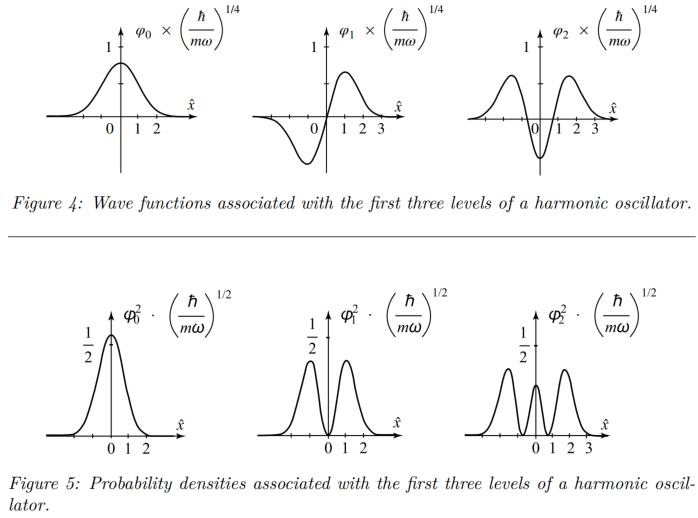
\includegraphics[width=.7\columnwidth]{PartOne/ChapterThree/excitedstatesqho.png}
\end{figure}



\section{Discussion}


\subsection{Mean values and rms eviations of $X$ and $P$ in a state $\ket{\varphi_n}$}

Neither $X$ nor $P$ comutes with $H$, and the eigenstates $\ket{\varphi_n}$ of $H$ are not eigenstates of $X$ or $P$. Consequently, if the harmonics oscillator is in stationary state $\ket{\varphi_n}$,
a measurement of the observable $X$ or $P$ can, a priori, yield any result.


We will compute the mean values of $X,P$ in such stationary state and also theirs rms deviation in order to set the uncertainty relation. 
We will use equations \eqref{eq:XPintermsofaa}, which show that neither $X$ nor $P$ has diagonal matrix elements:
\begin{align}
    \braket{\varphi_n|X|\varphi_n}=\braket{\varphi_n|P|\varphi_n}=0.
\end{align}
To obtain the rms deviations, we must calculate the mean value of $X^2$ and $P^2$. First, we note that 
\begin{align*}
    X^2&=\frac{\hbar}{2m\omega}(a^\dagger+a)(a^\dagger+a)=\frac{\hbar}{2m\omega}(a^{\dagger 2}+aa^\dagger+a^\dagger a+a^2)\\
    P^2&=-\frac{m\hbar\omega}{2}(a^\dagger-a)(a^\dagger-a)=-\frac{m\hbar\omega}{2}(a^{\dagger2}-aa^\dagger-a^\dagger a+a^2)
\end{align*}
The terms $a^2$ and $a^{\dagger2}$ do not contribute to the diagonal matrix elements, since $a^2\ket{\varphi_n}$ is proportional to $\ket{\varphi_{n-2}}$ and 
$a^{\dagger2}\ket{\varphi_n}$ to $\ket{\varphi_{n+2}}$; both are orthogonal to $\ket{\varphi_n}$. The rest of the terms yields:
\begin{align*}
    \braket{\psi_n|(a^\dagger a+aa^\dagger)|\varphi_n}=\braket{\varphi_n|(2a^\dagger a+1)|\varphi_n}=2n+1.
\end{align*}
Therefore, we have:
\begin{align}
    (\Delta X)^2&=\braket{\varphi_n|X|\varphi_n}-\braket{\varphi_n|X^2|\varphi_n}=\braket{\varphi_n|X^2|\varphi_n}=\left(n+\frac{1}{2}\right)\frac{\hbar}{m\omega}=\sigma^2\left(x+\frac{1}{2}\right).\\
    (\Delta P)^2&=\braket{\varphi_n|P|\varphi_n}-\braket{\varphi_n|P^2|\varphi_n}=\braket{\varphi_n|P^2|\varphi_n}=\left(n+\frac{1}{2}\right)m\hbar\omega=\frac{\hbar^2}{\sigma^2}\left(x+\frac{1}{2}\right).
\end{align}
The product is therefore 
\begin{align}
    \text{Uncertainty relation}\qquad\highlight{\Delta X\Delta P=\left(n+\frac{1}{2}\right)\hbar}.
\end{align}
We see that the lower bound is attained for $n=0$, that is, for the ground state.

\subsection{Properties of the ground state}
In classical mechanics, the lowest energy of the harmonic oscilaltor is obtained when the particle is at rest. In QM, the moninum energy sate is $\ket{\varphi_0}$, whose energy 
is not zero, and the associates wave function has a certain spatial extension, characterized by the rms deviation $\Delta X=\sqrt{\hbar/2m\omega}$.
The ground state correesponds to a compromie in which the sum of the kinetic and potential energy is as small as possible (uncertainty limitation).

\begin{emphasizer}
    The QHO possesses the peculiarity that due to the form of $V(x)$, the $\Delta X\Delta P$ attains its lower value at the ground state $\ket{\varphi_0}$. This is related to 
    the fact that the wave function of the ground state is Gaussian.
\end{emphasizer}

%%
\subsection{Time evolution of the mean values}
Consider thw state at $t=0$ 
\begin{align*}
    \ket{\psi(0)}=\sum_{n=0}^\infty c_n(0)\ket{\varphi_n}.
\end{align*}
Its state $\ket{\psi(t)}$ at $t$ can be obtained by using the evolution operator for conservative systems:
\begin{align}
    \ket{\psi(t)}=\sum_{n=0}^\infty c_n(0)e^{-iE_nt/\hbar}\ket{\varphi_n}=\sum_{n=0}^\infty c_n(0)e^{-i(n+1/2)\omega t}\ket{\varphi_n}.
\end{align}
The mean value of any physical quantity $A$ is 
\begin{align*}
    \braket{\varphi(t)|A|\varphi(t)}=\sum_{m,n=0}^\infty c_m^*(0)c_n(0)A_{mn}e^{i(m-n)\omega t},\quad\text{with}\quad A_{mn}=\braket{\varphi_m|A|\varphi_n}.
\end{align*}
The time evolution of the mean values involves only the frequency $\omega/2\pi$ and its various harmonics, which constitutes the Bohr frequencies of the harmonics oscillator.

If we consider $X$ and $P$, we know that the only non-zero elements $X_{mn}$ and $P_{mn}$ are those for which $m=n\pm1$. Consequently, the mean values of $X$ and $P$ include only terms in $e^{\pm\omega t}$.
Moreover, the form of the harmonics oscillator potential implies that for all $|ket{\varphi_n}$ the mean values of $X$ and $P$ rigorously satisfy the classical equations of motion. Using Ehrenfest theorem:
\begin{align}
    \begin{array}{l}
    \dfrac{d}{dt}\braket{X}=\dfrac{1}{i\hbar}\braket{[X,H]}=\dfrac{\braket{P}}{m}\\    
    \dfrac{d}{dt}\braket{P}=\dfrac{1}{i\hbar}\braket{[P,H]}=-m\omega^2\braket{X}
    \end{array}
    \stackrel{\int dt}{\longrightarrow}
    \begin{array}{l}
        \braket{X}(t)=\braket{X}(0)\cos\omega t+\dfrac{1}{m\omega}\braket{P}(0)\sin\omega t\\
        \braket{P}(t)=\braket{P}(0)\cos\omega t+m\omega\braket{X}(0)\sin\omega t
    \end{array}
\end{align}
\begin{itemize}[itemsep=0pt,topsep=0pt]
    \item In a stationary state $\ket{\varphi_n}$, the behavior of the harmonic oscillator is totally different from that predicted by classical mechanics. 
    The mean values of all the observables are constant over time.
\end{itemize}


%
\section{Stationary states in the $\{\ket{x}\}$ representation}
%%
\subsection{Hermite polynomials}

\subsubsection{Definition}
Let be the Gaussian function 
\begin{align}
    F(z)=e^{-z^2}
\end{align}
The successive derivatives are 
\begin{align*}
    F'(z)=-2ze^{-z^2},\quad F''(z)=(4z^2-2)e^{-z^2},\quad\cdots,\quad F^{(n)}(z)=(-1)^nH_n(z)e^{-z^2},
\end{align*}
where $H_n(z)$ is the nth-degree \bfemph{Hermite polynomial}:
\begin{align}
    \text{Hermite polynomial}\qquad\highlight{H_n(z)=(-1)^ne^{z^2}\frac{d^n}{dz^n}e^{-z^2}}.
\end{align}
The parity of $H_n(x)$ is $(-1)^n$, and it has $n$ real zeros between which one finds those of $H_{n-1}$.
\begin{figure}[h!]
    \centering
    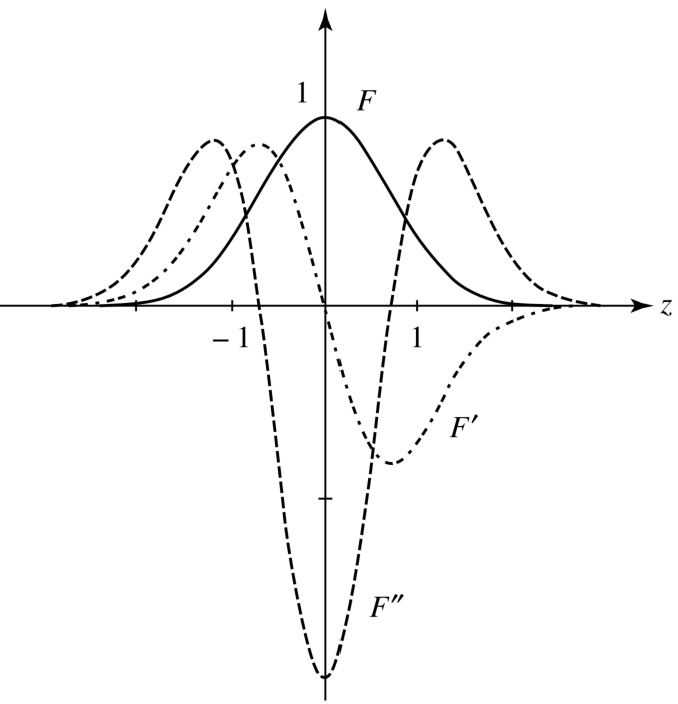
\includegraphics[width=.4\columnwidth]{PartOne/ChapterThree/gaussianandf.png}
    \caption{Shape of the Gaussian function $F(z)$ and its first and second derivatices.}
\end{figure}

\subsubsection{Generating function}



\subsubsection{Recurrence relations; differential equation}





%%
\subsection{The eigenfunctions of the harmonic oscillator Hamiltonian}

\subsubsection{Generating function}

\subsubsection{$\varphi_n(x)$ in terms of the Hermite polynomials}
What is $\varphi(x)=\braket{x|\varphi}$?

We know that $a\ket{\varphi_0}=0\ket{\varphi_0}$, so we replace the $\{\ket{x}\}$ representation 
\begin{align*}
    \braket{x|a|\varphi_0}=\braket{x|\frac{1}{\sqrt{2}}\left(\frac{x}{\sigma}+\frac{ip\sigma}{\hbar}\right)|\varphi_0}&=0\\
    \frac{1}{\sqrt{2}}\left(\frac{x}{\sigma}+\sigma\frac{\partial}{\partial x}\right)\varphi_0(x)&=\\
    \frac{\partial\varphi_0(x)}{\partial x}&=-\frac{x}{\sigma^2}\varphi_0(x).
\end{align*}
Its solution is 
\begin{align*}
    \varphi_0(x)=ce^{-\frac{x^2}{2\sigma^2}}\stackrel{\text{normalization}}{\longrightarrow}\varphi_0(x)=\left(\frac{1}{\pi\sigma^2}\right)^{1/4}e^{-\frac{x^2}{2\sigma^2}}.
\end{align*}

The general form is the following:
\begin{align}
    \text{Excited state in $\{\ket{x}\}$}\qquad\highlight{\varphi_n(x)=
    \left(\frac{\beta^2}{\pi}\right)^{1/4}\frac{1}{\sqrt{2^nn!}}e^{-\beta^2x^2/2}H_n(\beta x)}.
\end{align}
The shape of $\varphi_n(x)$ is therefore analogous to that of the nth-order derivative of the Gaussian function $F(x)$. Moreover, $\varphi_n(x)$ is of parity 
$(-1)^n$ and posseses $n$ zeros interposed between those of $\varphi_{n+1}(x)$. Recall this is related to the increase in the average kinetic energy of the 
states $\ket{\varphi_n}$ when $n$ increases.
%
\subsubsection{Recurrence relations}
Lets write the action of $a$ and $a^\dagger$ \eqref{eq:actionofaa} in the $\{\ket{x}\}$ representation. The action of them 
in this representation is 
\begin{align}
    a\longrightarrow \frac{\beta}{\sqrt{2}}\left[x+\frac{1}{\beta^2}\frac{d}{dx}\right]\qquad a^\dagger\longrightarrow\frac{\beta}{\sqrt{2}}\left[x-\frac{1}{\beta^2}\frac{d}{dx}\right].
\end{align}
Then equation \eqref{eq:actionofaa} becomes:
\begin{align}
    \text{Action of $a,a^\dagger$ in $\{\ket{x}\}$}\qquad\highlight{
        \begin{array}{l}
            \dfrac{\beta}{\sqrt{2}}\left[x+\dfrac{1}{\beta^2}\dfrac{d}{dx}\right]\varphi_n(x)=\sqrt{n}\varphi_{n-1}(x)\\\\
            \dfrac{\beta}{\sqrt{2}}\left[x-\dfrac{1}{\beta^2}\dfrac{d}{dx}\right]\varphi_n(x)=\sqrt{n+1}\varphi_{n+1}(x)
        \end{array}}
\end{align}

Taking the sum and difference:
\begin{align*}
    \begin{array}{l}
        x\beta\sqrt{2}\varphi_n(x)=\sqrt{n}\varphi_{n-1}(x)+\sqrt{n+1}\varphi_{n+1}(x)\\
        \dfrac{\sqrt{2}}{\beta}\dfrac{d}{dx}\varphi_n(x)=\sqrt{n}\varphi_{n-1}(x)-\sqrt{n+1}\varphi_{n+1}(x)
    \end{array}
\end{align*}
Replacing in them the function $\varphi_n(x)$ of equation x yields two recursive equations for $H(x)$ (setting $\hat{x}=\beta x$):
\begin{align*}
    \begin{array}{l}
        2\hat{x}H_n(\hat{x})=2nH_{n-1}(\hat{x})+H_{n+1}(\hat{x})\\
        2\left[-\hat{x}H_n(\hat{x})+\dfrac{d}{d\hat{x}}H_n(\hat{x})\right]=2nH_{n-1}(\hat{x})-H_{n+1}(\hat{x})
    \end{array}
\end{align*}
\section{The isotropic three-dimensional harmonic oscillator}
\section{Coherent states of the harmonic oscillator}
We know that quantum mechanics must yield the same results as classical mechanics in the limiting casr where the harmonic 
oscillator has an energy much greater than the quantum $\hbar\omega$.

It is possible to construct quantum mechanics states leading to physical predictions which are almost identical to the classical ones, at least 
for a macroscopic oscillator? Such quantum sistems do exist: they are coherent linear superpositions of all the states $\ket{\varphi_n}$. We shall 
call them \bfemph{quasi-classical states} or coherent states of the harmonic oscillator.

It is important to understand, in the framework of quantum mechanics, how to move gradually from the case in which thee results given by the classical approximation 
are sufficient to the case in which quantum effects are preponderant.

The position, momentum, and energy of a harmonic oscillator are described in QM by operators which do not commute.
It is not possible to construct a state in which they are all perfectly well-defined.

Theregore, we shall only look for a state vector such that for all $t$, the mean values $\braket{X}$, $\braket{P}$, and $\braket{H}$ are 
as close as possible to the corresponding classical values: the compromise if then that none of these three observables is perfectly known.
Nevertheless, the rms deviation $\Delta X$, $\Delta Y$, and $\Delta H$ are, in the macroscopic limit, completely negligible.
%%
\subsection{Quasi-classical states}
%
\subsubsection{Introducing $\alpha_0$ to characterize a classical motion}
The classical quantitites of motion of a 1D harmonics oscillator of mass $m$ and angular frrequency $\omega$ are 
\begin{align}
    \text{Equations of motion for CHO}\qquad\highlight{\begin{array}{l}
        \dfrac{d}{dt}x(t)=\dfrac{1}{m}p(t)\\
        \dfrac{d}{dt}p(t)=-m\omega^2x(t)
    \end{array}}.
\end{align}
The classical state of the HO is determined at time $t$ when we know its position $x(t)$ and its momentum $p(t)$.
We shall therefore combine them into a single complex number $\alpha(t)$ given by:
\begin{align}
    \text{Displacement coordinate}\qquad\highlight{\alpha(t)=\frac{1}{\sqrt{2}}\left(\frac{x(t)}{\sigma}+i\frac{\sigma p(t)}{\hbar}\right)\quad(-)}.
\end{align}
Then, the equations of motions turn to 
\begin{align}
    \frac{d}{dt}\alpha(t)=-i\omega\alpha(t)\longrightarrow\highlight{\alpha(t)=\alpha_0e^{-i\omega t},\quad \alpha_0=\alpha(0)}
    \label{eq:timeevolaclassic}
\end{align}
We can plot this evolution in a geometrical representation of the evolution of the state of the system through the \bfemph{phase-space diagram} 
as shown in the following figure.
\begin{figure}[h!]
    \centering
    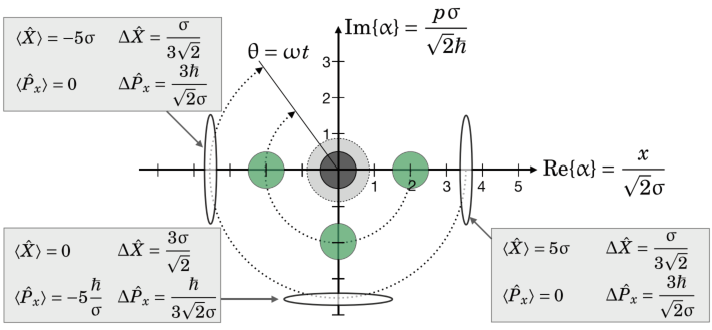
\includegraphics[width=.7\columnwidth]{PartOne/ChapterThree/phasespacediagram.png}
    \caption{Illustration of four HO states in the phase-space diagram: black=ground state, gray=first excited state, 
    ovals=squeezed state, green=coherent state.}
\end{figure}
According to the solution of the ODE, we have 
\begin{align}
    x(t)=\frac{1}{\sqrt{2}}(\alpha_0e^{-i\omega t}+\alpha_0^*e^{i\omega t}),\quad p(t)=-\frac{i}{\sqrt{2}}(\alpha_0e^{-i\omega t}-\alpha_0^*e^{i\omega t}).
\end{align}
As for the classcal energy $\mathcal{H}$ of the system, it is constant in time and equal to:
\begin{align*}
    \mathcal{H}=\frac{1}{2m}p(0)^2+\frac{1}{2}m\omega^2x^2(0)=\frac{\hbar\omega}{2}\left[\left(\frac{x(0)}{\sigma}\right)^2+\left(\frac{\sigma p(0)}{\hbar}\right)^2\right]=\hbar\omega|\alpha_0|^2.
\end{align*}
For a macroscopic oscillator, the energy $\mathcal{H}$ is much greater than the quantum $\hbar\omega$, so 
\begin{align}
    \text{Macroscopic regime}\qquad\highlight{|\alpha_0|\gg1}.
\end{align}


%
\subsubsection{Conditions defining quasi-classical states}
We are looking for a quantum mechanical state for which at every instant the mean values $\braket{X}$, $\braket{P}$, and $\braket{H}$ are practically equal to the values of 
$x$, $p$, and $\mathcal{H}$ which correspond to a given classical motion.

The time evolution of the matrix element $\braket{a}(t)=\braket{\psi(t)|a|\psi(t)}$ is given by 
\begin{align*}
    i\hbar\partial_t\braket{a}(t)=\braket{[a,H]}(t)
\end{align*}
The commutator is $[a,H]=[a,a^\dagger a]=\hbar\omega a$, which implies that the solution of the above ODE is 
\begin{align}
    \braket{a}(t)=\braket{a}(0)e^{-i\omega t}.
    \label{eq:timeevolutiona}
\end{align}
The evolution of $\braket{a^\dagger}(t)$ satisfies the adjoint equation:
\begin{align*}
    \braket{a^\dagger}(t)=\braket{a^\dagger}(0)e^{i\omega t}=\braket{a}^*(0)e^{i\omega t}.
\end{align*}
The equation \eqref{eq:timeevolutiona} is anaologous to equation \eqref{eq:timeevolaclassic}. We can substitute $\braket{a}(t)$ and $\braket{a^\dagger}(t)$ in 
the mean value of $X$ and $P$ to get:
\begin{align}
    \braket{X}(t)&=\frac{1}{\sqrt{2}}(a+a^\dagger)=\frac{1}{\sqrt{2}}[\braket{a}(0)e^{-i\omega t}+\braket{a}^*e^{i\omega t}]\\
    \braket{P}(t)&=\frac{i}{\sqrt{2}}(a^\dagger-a)=\frac{i}{\sqrt{2}}[\braket{a}^*e^{i\omega t}-\braket{a}(0)e^{-i\omega t}]
\end{align}
It is necessary and sufficient to set at $t=0$ the condition $\braket{a}(0)=\alpha_0$, which resembles to the classical motion. The normalized state vector $\ket{\psi(t)}$ of the oscillator 
must therefore satisfy the condition 
\begin{align*}
    \text{First condition}\qquad\braket{\psi(0)|a|\psi(0)}=\alpha_0.
\end{align*}
We must now require the mean value 
\begin{align}
    \braket{H}=\hbar\omega\braket{a^\dagger a}(0)+\frac{\hbar\omega}{2}
\end{align}
to be equal to the classical energy $\mathcal{H}$. Given that for a classical oscillator $|\alpha_0|$ is much greater than $1$, we shall neglect the term $\hbar\omega/2$ with respect to 
$\hbar\omega|\alpha_0|^2$. The second condition on the state vector can now be written:
\begin{align}
    \text{Second condition}\qquad\braket{\psi(0)|a^\dagger a|\psi(0)}=|\alpha_0|^2.
\end{align}
The two conditions are sufficient to determine the normalized state vector $\ket{\psi(0)}$.
%
\subsubsection{Quasi-classical states are eigenvectors of the operator $a$}
If a normalized vector $\ket{\psi(0)}$ satisfy the relation 
\begin{align}
    a\ket{\psi(0)}=\alpha_0\ket{\psi(0)},
    \label{eq:twoconditionsequation}
\end{align}
then the two conditions above are satisfied.
%
The quasi-classical state, associated with a classical motion characterized by the parameter $\alpha_0$ is such that $\ket{\psi(0)}$ is an eigenvector of the operator 
$a$ with the eigenvalue $\alpha_0$. We will denote the eigenvector of $a$ with eigenvalue $\alpha$ by $\ket{\alpha}$:
\begin{align}
    \text{Eigenvector of $a$ with eigenvalue $\alpha$}\qquad a\ket{\alpha}=\alpha\ket{\alpha}.
    \label{eq:eigenvectoralpha}
\end{align}
%%
\subsection{Properties of the $\ket{\alpha}$ states}
%
\subsubsection{Expansion of $\ket{\alpha}$ on the basis of the stationary states $\ket{\varphi_n}$}
Let us determine the ket $\ket{\alpha}$ wich is a solution of \eqref{eq:twoconditionsequation} by using an expansion on $\ket{\varphi_n}$:
\begin{align*}
    \ket{\alpha}=\sum_nc_n(\alpha)\ket{\varphi_n}.
\end{align*}
We then have 
\begin{align*}
    a\ket{\alpha}=\sum_nc_n(\alpha)\sqrt{n}\ket{\varphi_{n-1}}
\end{align*}
and, substituting this into \eqref{eq:eigenvectoralpha} yields 
\begin{align*}
    c_{n+1}(\alpha)=\frac{\alpha}{\sqrt{n+1}}c_n(\alpha).
\end{align*}
This relation enable us to determine by recurrence all the coefficient $c_n(\alpha)$ in terms of $c_0(\alpha)$:
\begin{align}
    c_n(\alpha)=\frac{\alpha^n}{\sqrt{n!}}c_0(\alpha).
\end{align}
When $c_0(\alpha)$ is fixed, all the $c_n(\alpha)$ are also fixed. The vectoer $\ket{\alpha}$ is therefore unique. We shall choose $c_0(\alpha)$ real, positive and 
normalized with $\ket{\alpha}$, which determines it completely:
\begin{align}
    \sum_n|c_n(\alpha)|^2=|c_0(\alpha)|^2\sum_n\frac{|\alpha|^{2n}}{n!}=|c_0(\alpha)|^2e^{|\alpha|^2}=1.
\end{align}
We the convenction we have chosen we have $c_0(\alpha)=e^{-|\alpha|^2/2}$ and finally,
\begin{align}
    \ket{\alpha}=e^{-|\alpha|^2/2}\sum_n\frac{\alpha^n}{\sqrt{n!}}\ket{\varphi_n}.
    \label{eq:alphaket}
\end{align}
This result was also obtained by Cris displacing the $\ket{\varphi_0}$ from the origin by $x_0$ (lecture 14). It began with $\ket{\psi}=S(x_0)\ket{\varphi_0}$ and got some expression.
Then, we replaced $\ket{\psi}$ by $\ket{\alpha}$ with the corresponding transformation: $\alpha=x_0/(\sqrt{2}\sigma)$.
%
\subsubsection{Possible values of the energy in an $\ket{\alpha}$ state}
Assuming an oscillator in the state $\ket{\alpha}$, we see from \eqref{eq:alphaket} that a measurement of the energy can yield the result $E_n=(n+1/2)\hbar\omega$ with the probability:
\begin{align}
    \text{Probability of having $E_n$}\qquad\highlight{P_n(\alpha)=|\braket{\alpha|\varphi_n}|^2=\frac{|\alpha|^{2n}}{n!}e^{-|\alpha|^2}}.
\end{align}
The probability obtained corresponds to a \bfemph{Poisson distribution}. We have from its a recurrence relation:
\begin{align*}
    P_n(\alpha)=\frac{|\alpha|^2}{n}P_{n-1}(\alpha).
\end{align*}
$P_n(\alpha)$ reaches its maximum when $n$ is the integral part of $|\alpha|^2$.
%
\subsubsection{Calculation of mean values and uncertainties}
The mean value can be obtaines expressing them in terms of the $a$ operators, and using \eqref{eq:alphaket}:
\begin{align}
    \begin{array}{l}
    \braket{X}_\alpha=\braket{\alpha|X|\alpha}=\sqrt{2}\sigma\re{\alpha},\quad\braket{X^2}_\alpha=\frac{\sigma^2}{2}[(\alpha+\alpha^*)^2+1]\\
    \braket{P}_\alpha=\braket{\alpha|P|\alpha}=\frac{\sqrt{2}\hbar}{\sigma}\im{\alpha},\quad\braket{P^2}_\alpha=\frac{m\hbar\omega}{2}[1-(\alpha-\alpha^*)^2]\\
    \braket{N}_\alpha=\braket{\alpha|N|\alpha}=|\alpha|^2,\quad\braket{N^2}_\alpha=-\\
    \braket{H}_\alpha=\braket{\alpha|H|\alpha}=\hbar\omega\left[|\alpha|^2+\frac{1}{2}\right],\quad\braket{H^2}_\alpha=\hbar^2\omega^2\left[|\alpha|^4+2|\alpha|^2+\frac{1}{4}\right]
    \end{array}
    \label{eq:meanvalues}
\end{align}
Therefore, we have:
\begin{align}
    \Delta X_\alpha=\frac{\sigma}{\sqrt{2}},\quad\Delta P_\alpha=\frac{\hbar}{\sqrt{2}\sigma},\quad\Delta N_\alpha=|\alpha|,\quad\Delta H_\alpha=\hbar\omega|\alpha|.
\end{align}
The $XP$ uncertainty relation is therefore:
\begin{align}
    \Delta X_\alpha\Delta P_\alpha=\frac{\hbar}{2}.
\end{align}
%
\subsubsection{The displacement operator $D(\alpha)$}
Let be the operator define by 
\begin{align}
    \text{Displacement operator}\qquad\highlight{D(\alpha)=T(\braket{X})S(\braket{P})e^{i\braket{X}\braket{P}/\hbar}=e^{\alpha a^\dagger-\alpha^*a}}.
\end{align}
This operator is unitary since 
\begin{align*}
    D^\dagger(\alpha)=e^{\alpha^*a-\alpha a^\dagger}\Longrightarrow D(\alpha)D^\dagger(\alpha)=D^\dagger(\alpha)D(\alpha)=1.
\end{align*}
The argument of the exponential can be defined with the commutator $[\alpha a^\dagger,-\alpha^* a]=\alpha^*\alpha$ so that using the Glauber formula for exponential 
yields:
\begin{align*}
    D(\alpha)=e^{-|\alpha|^2/2}e^{\alpha a^\dagger}e^{-\alpha^*a}
\end{align*}
Now, the action of $D(alpha)$ into a ket $\ket{\varphi_0}$ can be considerd by parts. First,
\begin{align*}
    e^{-\alpha^*a}\ket{\varphi_0}=\left[1-\alpha^*a+\frac{\alpha^{*2}}{2!}a^2+\cdots\right]\ket{\varphi_0}=\ket{\varphi_0}.
\end{align*}
Because it returns the same ket, we are left with the second exponential:
\begin{align*}
    D(\alpha)\ket{\varphi_0}=e^{-|\alpha|^2/2}e^{\alpha a^\dagger}\ket{\varphi_0}=e^{-|\alpha|^2/2}\sum_n\frac{(\alpha a^\dagger)^n}{n!}\ket{\varphi_0}=e^{-|\alpha|^2/2}\sum_n\frac{\alpha^n}{\sqrt{n!}}\ket{\varphi_n}.
\end{align*}
Comparing with \eqref{eq:alphaket} we have 
\begin{align}
    \ket{\alpha}=D(\alpha)\ket{\varphi_0}.
\end{align}
$D(\alpha)$ is therefore the unitary transformation which transforms the ground state $\ket{\varphi_0}$ into the quasi-classical state $\ket{\alpha}$.
This was that cris derived but for only a position displacement.
\begin{example}{Translation with D}
    Let be 
    \begin{align*}
        D(\alpha)=e^{\frac{1}{\sqrt{2}}(5+10i)a^\dagger-\frac{1}{\sqrt{2}}(5-10i)a}.
    \end{align*}
    We identify $\alpha=5+10i$ and $\alpha^*=5-10i$. Using the result of mean values \eqref{eq:meanvalues} we have 
    \begin{align*}
        \braket{X}=5\sigma,\quad\text{and}\quad\braket{P}=\frac{10\hbar}{\sigma}.
    \end{align*}
    Then,
    \begin{align*}
        \varphi_0(x)=\left(\frac{1}{\pi\sigma^2}\right)^{1/4}e^{-x^2/2\sigma^2}\Longrightarrow\braket{x|D|\varphi_0}=\left(\frac{1}{\pi\sigma^2}\right)^{1/4}e^{i\dfrac{x}{\hbar}\left(10\dfrac{\hbar}{\sigma}\right)}e^{-\dfrac{(x-5\sigma)^2}{2\sigma^2}}.
    \end{align*}
\end{example}
%
\subsubsection{Scalar product of two $\ket{\alpha}$ states. Closure relation}
The $\ket{\alpha}$ states are eigenvectors of the non-Hermitian operator $a$. There is therefore no obvious reason for these states to satisfy orthogonality 
and closure relation.

The scalar product between $\ket{\alpha}$ and $\ket{\alpha'}$ is:
\begin{align*}
    \braket{\alpha|\alpha'}=\sum_n c_n^*(\alpha)c_n(\alpha')=e^{-|\alpha|^2/2}e^{-|\alpha'|^2/2}\sum_n\frac{(\alpha^*\alpha')^n}{n!}=e^{-|\alpha|^2/2}e^{-|\alpha'|^2/2}e^{\alpha^*\alpha'}.
\end{align*}
That is,
\begin{align}
    \text{Orthonormalization relation}\qquad|\braket{\alpha|\alpha'}|^2=e^{-|\alpha-\alpha'|^2}.
\end{align}
We see that \textbf{they are not orthogonal}, unless $\alpha=\alpha'$.

However, \textbf{they do satisfy the closure relation}:
\begin{align*}
    \frac{1}{\pi}\iint\ket{\alpha}\bra{\alpha}\;d\{\re{\alpha}\}d\{\im{\alpha}\}=\cdots=\sum_n\ket{\varphi_n}\bra{\varphi_n}=1.
\end{align*}

%%
\subsection{Time evolution of a quasi-classical state}
Given the initial state $\ket{\psi(0)}=\ket{\alpha_0}$, How do its physical properties evolve over time? 
%
\subsubsection{A quasi-classical state always remains an eigenvector of $a$}
We use the time eovlution assuming conservative system (Hamiltonian time-independent)
\begin{align*}
    \ket{\psi(t)}&=e^{-iE_nt/\hbar}\ket{\alpha_0}=e^{-i\omega t(a^\dagger a+1/2)}\ket{\alpha_0}=e^{-i\omega t/2}e^{-i\omega t \underbrace{a^\dagger a}_{N}}\ket{\alpha_0}=e^{-i\omega t/2}e^{-i\omega tN}\ket{\alpha_0}\\
    &=e^{-i\omega t/2}e^{-i\omega tN}e^{-\frac{|\alpha|^2}{2}}\sum_{n=0}^\infty\frac{\alpha_0^n}{\sqrt{n!}}\ket{n}=e^{-i\omega t/2}e^{-\frac{|\alpha|^2}{2}}\sum_{n=0}^\infty\frac{\alpha_0^n}{\sqrt{n!}}e^{-i\omega tN}\ket{n}\\
    &=e^{-i\omega t/2}e^{-\frac{|\alpha|^2}{2}}\sum_{n=0}^\infty\frac{1}{\sqrt{n}}(\alpha_0e^{-i\omega t})^n\ket{n}=e^{-i\omega t/2}\ket{\alpha_0e^{-i\omega t}}=e^{-i\omega t/2}\ket{\alpha(t)}.
\end{align*} 
Thus, we have found that 
\begin{align}
    \text{Evolution of the quasi-classical state}\qquad\highlight{\ket{\psi(t)}=e^{-\frac{i\omega t}{2}}\ket{\alpha(t)=\alpha_0e^{-i\omega t}}}.
    \label{eq:evolcoherentstate}
\end{align}
We see that a quasi-classical state remains an eigenvector of $a$ for all time, with an eigenvalue $\alpha_0e^{-i\omega t}$ which is nothing more than $\alpha(t)$ obtained at the begining.
%
\subsubsection{Evolution of physical properties}
We use equation \eqref{eq:meanvalues} and change $\alpha$ by $\alpha_0e^{-i\omega t}$ to obtain:
\begin{align}
    \text{Mean values for $\alpha(t)$}\qquad\highlight{\begin{array}{l}
        \braket{X}(t)=\sqrt{2}\sigma\re{\alpha(t)}\\
        \braket{P}(t)=\frac{\sqrt{2}\hbar}{\sigma}\im{\alpha(t)}\\
        \braket{N}=|\alpha|^2\\
        \braket{H}=\hbar\omega[|\alpha_0|^2+\frac{1}{2}]
    \end{array}}
\end{align}
And the corresponding uncertainties are:
\begin{align}
    \text{Uncertainties}\qquad\begin{array}{l}
        \Delta X=\frac{\sigma}{\sqrt{2}}\\
        \Delta P=\frac{\hbar}{\sqrt{2}\sigma}\\
        \Delta H=\hbar\omega|\alpha_0|
    \end{array}
\end{align}
The uncertainty relation holds: 
\begin{align*}
    \Delta X\Delta P=\frac{\hbar}{2}.
\end{align*}
Using the above mean values, we express $\alpha(t)$ as:
\begin{align}
    \highlight{\alpha(t)=\frac{1}{\sqrt{2}}\left[\frac{\braket{X}(t)}{\sigma}+i\frac{\sigma\braket{P}(t)}{\hbar}\right]}.
\end{align}
%
\subsubsection{Motion of the wave packet}
Let us calculate the wave function $\psi(x,t)$. Using \eqref{eq:evolcoherentstate} and (76), we have:
\begin{align*}
    \psi(x,t)=e^{i\theta_\alpha}\left(\frac{1}{\pi\sigma^2}\right)^{1/4}e^{-i\omega t/2}e^{-\frac{x\braket{P}(t)}{\hbar}}e^{-\left[\frac{x-\braket{x}(t)}{2\Delta X}\right]^2}.
\end{align*}
At $t$, the wave packet is still Gaussian. Thus, it remains minimum for all time. THe following figure shows the motion of the wave packe, performing periodc oscillation withouth becoming distorted.
In free particle, this type of wave packer would become distorted as it propagates, but here the potential compensates that spreading so that the shape is always the same.
\begin{figure}[h!]
    \centering
    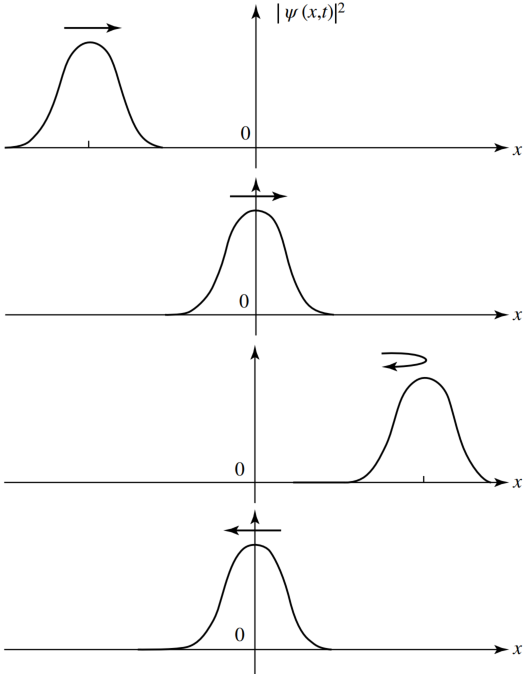
\includegraphics[width=.4\columnwidth]{PartOne/ChapterThree/gaussianalphastate.png}
    \caption{Motion of the Gaussian wave packet associated with $\ket{\alpha}$ state. Thanks to the form of $V(x)$, the wave packet oscillates without distortion.}
\end{figure}

% bibliography
\newpage
%\section*{Bibliography}
%
\begin{refsection}
    \nocite{*}
    %
    \subsection*{Mathematics}
    \printbibliography[heading=none,title={}, keyword=bib_template]
    %

    %
\end{refsection}